
\subsection{Complexity Analysis}
In this section, we will try to provide an upper bound estimation about space and runtime of our proposed solutions. It is difficult to provide the exact complexity because of having different types of parameters, e.g., input threshold, data characteristics, etc. For both solutions, first we will introduce the used terminologies, then the upper bound complexities along with a small description about the reduction from the upper bounds. 

\subsubsection{Tree-Miner with SP-Tree}
We have tried to maintain the consistency in variables declaration throughout the study. In Table \ref{table:variables_complexity_tree_miner}, we have listed down the essential and additional variables used in this discussion. In Table \ref{table:space_complexity_tree_miner} and Table \ref{table:runtime_complexity_tree_miner}, we have summarized our discussion to indicate memory and runtime complexity for the proposed static solution respectively. We have shown the upper bound values and practically the value is much lesser due to different criterion. 


\begin{table}
\parbox{.49\linewidth}{
\centering
\begin{tabular}{|c|c|}
\hline
Name & Variables\\
\hline
Length of $s_{i}$ & $L_{i}$ \\ \hline
Number of nodes  & $N$ \\ 
of SP-Tree & \\ \hline
Average number of  & $u_{i}$ \\
unique symbols in the & \\ 
subtree of each node &  \\ \hline
Total number of & $I$ \\ 
unique symbols & \\ 
\hline
Average number of  &  $k$ \\ 
unique symbols in & \\
each sequence & \\ \hline
Total number of  & $Z$ \\ 
patterns tested & \\
\hline
Average Projection cost & $S^{*}$ \\ \hline
\end{tabular}
\caption{Additional Variables used in complexity discussion: static solution}
\label{table:variables_complexity_tree_miner}
}
\hfill
\parbox{.49\linewidth}{
\centering
\begin{tabular}{|c|c|}
\hline
Name & Variables\\
\hline
Number of nodes of  & $N^{\prime}$ \\ 
IncSP-Tree & \\ 
\hline
Modified nodes of  & $M$ \\ 
IncSP-Tree & \\ 
\hline
Unmodified nodes of  & $U$ \\ 
IncSP-Tree & \\ 
\hline
Average number of modified  & $\widetilde{u}$ \\ 
unique symbols in the & \\ 
subtree of each  &  \\ 
modified node & \\ 
\hline
Total number of  & $I$ \\ 
unique symbols & \\ 
\hline
Average number of  &  $k$ \\ 
unique symbols for & \\ 
each sequence of $D$ & \\ 
\hline
Average number of & $\widetilde{k}$  \\ 
 unique symbols for & \\ 
each sequence of $db$ &  \\ 
\hline
Total number of  & $Z_{F}$ \\ 
frequent patterns & \\ 
\hline
Number of nodes & $|B|$ \\ 
in BPFSP-Tree & \\ 
\hline
\end{tabular}
\caption{Additional Variables used in complexity discussion: incremental solution}
\label{table:variables_complexity_inc_tree_miner}
}
\end{table}

\begin{table}[!t]
%% increase table row spacing, adjust to taste
%\renewcommand{\arraystretch}{1.3}
% if using array.sty, it might be a good idea to tweak the value of
% \extrarowheight as needed to properly center the text within the cells

\centering
%% Some packages, such as MDW tools, offer better commands for making tables
%% than the plain LaTeX2e tabular which is used here.
\begin{tabular}{|c|c|c|}
\hline
Structural Elements & Upper Bounds & Reasoning\\
\hline
$N$  & $\sum_{i=1}^{|D|} L_{i}$ & $N << \sum_{i=1}^{|D|} L_{i}$ Due to \\
& & node overlapping \\ \hline
Total Cost related to $next\_link$ & $\mathcal{O}(u_{i} \times N)$ & Due to link based\\
& & implementation and node overlapping,\\
& & the value will reduce.\\ \hline
Co-Existing Item Table & $\mathcal{O}(I^{2})$ & Only the found combinations \\
& & are stored. \\ \hline
Sequence Summarizer & $\mathcal{O}(|D| \times k)$ & Sequence length, number of unique \\
& & symbols in each sequence \\
& & dominate this.\\ 
\hline
\end{tabular}
\caption{Static solution's upper bound space complexity}
\label{table:space_complexity_tree_miner}
\end{table}

\begin{table}[!t]
%% increase table row spacing, adjust to taste
%\renewcommand{\arraystretch}{1.3}
% if using array.sty, it might be a good idea to tweak the value of
% \extrarowheight as needed to properly center the text within the cells
\centering
%% Some packages, such as MDW tools, offer better commands for making tables
%% than the plain LaTeX2e tabular which is used here.
\begin{tabular}{|c|c|c|}
\hline
Function & Upper Bounds & Reasoning\\
\hline
Sequence Insertion &  $\sum_{i=1}^{|D|}L_{i}$ & -  \\ \hline
Node  & $\mathcal{O}(N \times u_{i})$ & Same nodes' attributes does\\ 
attributes & & not need to be \\
calculation & & calculated twice\\ 
\hline
$CETable$  & $\mathcal{O}(|D| \times k^{2})$ & Depends on unique number \\ 
calculation & & of symbols for\\
& & each sequence\\
\hline
Pre-processing & $\sum_{i=1}^{|D|}L_{i}$ +  & - \\ 
Complexity & $\mathcal{O}(|D| \times k^{2})$ + & \\ 
&  $\mathcal{O}(N \times u_{i})$ & \\ 
\hline 
Pattern Projection  & $\mathcal{O}(S_{P})$ & Due to Breadth-First support \\ 
Complexity of $P$ & & counting technique \\ 
& & and node overlapping.\\ 
\hline
Total  &  $\mathcal{O}(Z \times S^{*})$ & Number of patterns searching \\ 
Mining &  $Z << (2^{T}-1)^{E}$ & get reduced through applying \\ 
Complexity & $S^{*} << \frac{S_{P_{1}}+S_{P_{2}}+S_{P_{3}}+...+S_{P_{Z}}}{Z}$ & different pruning strategies.\\ 
\hline
\end{tabular}
\caption{Static solution's upper bound runtime complexity}
\label{table:runtime_complexity_tree_miner}
\end{table}

\subsubsection{IncTree-Miner with IncSP-Tree}
Similar to previous discussion, the additional variables to discuss the upper bound complexity of the proposed incremental solution is stated in Table \ref{table:variables_complexity_inc_tree_miner}. The upper bound space and runtime complexities of our incremental solution along with a discussion about the possibilities of reduced complexities in average scenarios is stated in Table \ref{table:space_complexity_inc_tree_miner} and \ref{table:table_complexity_incremental}, \ref{table:runtime_complexity_inc_tree_miner} respectively. If, we want to store the projection information in the BPFSP-Tree, we need to store the support and projection nodes for each pattern and in the memory resilient version, we just only store the support information. In Table \ref{table:table_complexity_incremental}, we have shown the runtime upper bound complexities of different types of projection cases. Our incremental algorithm first perform projection in the modified subtrees, tests the infrequent to frequent property and based on that perform projection in the unmodified subtrees. The complexities mainly reduce by identifying the infrequent patterns early through breadth-first technique.  

\begin{table}[!t]
%% increase table row spacing, adjust to taste
%\renewcommand{\arraystretch}{1.3}
% if using array.sty, it might be a good idea to tweak the value of
% \extrarowheight as needed to properly center the text within the cells
\centering
%% Some packages, such as MDW tools, offer better commands for making tables
%% than the plain LaTeX2e tabular which is used here.
\begin{tabular}{|c|c|c|}
\hline
Structural Elements & Upper Bounds & Reasoning\\
\hline
Number of modified  & $|M| = \sum_{i=1}^{|db|} (L_{i}^{D}+L_{i}^{db})$ & Node overlapping\\ 
nodes of IncSP-Tree & & \\ 
\hline
Total number of   & $N^{\prime}=|U|+|M|$ & Node overlapping\\ 
nodes of IncSP-Tree & & \\ 
\hline
Total Cost related to & $\mathcal{O}(u_{i} \times N^{\prime})$ & Database characteristics, link  \\ 
$next\_link$ & & based implementation, node\\ 
& & overlapping\\ 
\hline
Total Cost related to & $\mathcal{O}(\widetilde{u} \times M)$ & Database characteristics, link   \\ 
$modified\_next\_link$ & & based implementation, node  \\
& & overlapping, database \\ 
& & update feature  \\ 
\hline
Co-Existing  & $\mathcal{O}(I^{2})$ & Stated in Table \ref{table:space_complexity_tree_miner} \\ 
Item Table & & \\ 
\hline
Sequence Summarizer & $\mathcal{O}(|D^{\prime}| \times k)$ & Stated in Table \ref{table:space_complexity_tree_miner}\\ \hline
BPFPS-Tree with &  $\mathcal{O}(Z_{F} \times S^{*})$ & IncSP-Tree compact\\
projection information  & $S^{*} << \frac{S_{P_{1}}+S_{P_{2}}+S_{P_{3}}+...+S_{P_{Z_{F}}}}{Z_{F}}$ & node references\\
\hline
BPFPS-Tree with & $\mathcal{O}(Z_{F})$ & Only the support value\\ 
only support & & \\ 
\hline
\end{tabular}
\caption{Incremental solution's upper bound space complexity}
\label{table:space_complexity_inc_tree_miner}
\end{table}


\begin{table}[!t]
%% increase table row spacing, adjust to taste
%\renewcommand{\arraystretch}{1.3}
% if using array.sty, it might be a good idea to tweak the value of
% \extrarowheight as needed to properly center the text within the cells
\centering
%% Some packages, such as MDW tools, offer better commands for making tables
%% than the plain LaTeX2e tabular which is used here.
\begin{tabular}{|c|c|c|c|c|}
\hline
Serial & \textit{Old Status} & Infrequent to frequent & New status & Total\\
& \textit{in D}& property satisfied & in $D^{\prime}$ & Cost \\ 
\hline
1 & Frequent & Yes & Frequent & $\mathcal{O}($T_{P\gamma}^{M}$)$ \\ \hline
2 & Frequent & No & Infrequent & $\mathcal{O}($T_{P\gamma}^{M}$)$ \\ \hline
3 & Infrequent & No & Infrequent & $\mathcal{O}($T_{P\gamma}^{M}$)$ \\ 
 & ($S_{P\gamma}^{D} \in NIB$) & & &\\ \hline
4 & Infrequent & Yes &  Infrequent & $\mathcal{O}($T_{P\gamma}^{M}$)$ \\ 
 & ($S_{P\gamma}^{D} \in NIB$)  & & &\\ \hline
5 & Infrequent & Yes & Frequent & $\mathcal{O}($T_{P\gamma}^{M}$)+\mathcal{O}($T_{P\gamma}^{U}$)$ \\ 
 & ($S_{P\gamma}^{D} \in NIB$)  & & &\\ \hline
 6 & Infrequent & No & Infrequent & $\mathcal{O}($T_{P\gamma}^{M}$)$ \\ 
 & ($S_{P\gamma}^{D} \notin NIB$) & & &\\ \hline
7 & Infrequent & Yes &  Infrequent & $\mathcal{O}($T_{P\gamma}^{M}$)+\mathcal{O}($T_{P\gamma}^{U}$)$ \\ 
 & ($S_{P\gamma}^{D} \notin NIB$)  & & &\\ \hline
8 & Infrequent & Yes & Frequent & $\mathcal{O}($T_{P\gamma}^{M}$)+\mathcal{O}($T_{P\gamma}^{U}$)$ \\ 
 & ($S_{P\gamma}^{D} \notin NIB$)  & & &\\ \hline
\end{tabular}
\caption{Projection runtime Complexities during different types of pattern transitions from $P$ to $P\gamma$}
\label{table:table_complexity_incremental}
\end{table}


\begin{table}[!t]
\small
%% increase table row spacing, adjust to taste
%\renewcommand{\arraystretch}{1.3}
% if using array.sty, it might be a good idea to tweak the value of
% \extrarowheight as needed to properly center the text within the cells
\centering
%% Some packages, such as MDW tools, offer better commands for making tables
%% than the plain LaTeX2e tabular which is used here.
\begin{tabular}{|l|l|l|}
\hline
Function & Upper Bounds & Reasoning \\
\hline
Sequence &  $\sum_{i=1}^{|db|}L_{i}^{db}$ & -\\ 
Insertion  & & \\ 
\hline
Node  & $\mathcal{O}(\widetilde{u} \times \{ \sum_{i=1}^{|db|} L_{i}^{db}+L_{i}^{D}\})$ & One time update  \\ 
attributes & & for an overlapped \\ 
 Update & & modified node\\ 
 \hline
$CETable$ & $\mathcal{O}(|db| \times k \times \widetilde{k})$ & Only the \\ 
Update & & unique symbols.\\ 
\hline
Pre- & $\sum_{i=1}^{|db|}L_{i}^{db}$ + $\mathcal{O}(\widetilde{u}  \times \{ \sum_{i=1}^{|db|} L_{i}^{db}+L_{i}^{D} \} )$ + $\mathcal{O}(|db| \times k \times \widetilde{k})$ & -\\ 
processing & & \\ 
Complexity & & \\ 
 \hline 
Total &  $\mathcal{O}(|Z| \times S^{*})$ & Pattern searching  \\ 
Mining  &  $Z << (2^{T}-1)^{E}$ & space is reduced \\ 
Complexity & $S^{*} \textless \textless \frac{\sum_{P\in Z_{1}} T_{P}^{M} + ...+\sum_{P\in Z_{8}} T_{P}^{M}+T_{P}^{U} + \sum_{P \in Z_{Prune}} |P| + |B| }{|Z|}$ & due to different\\
& & strategies. \\ 
\hline
\end{tabular}
\caption{Incremental solution's upper bound runtime complexity}
\label{table:runtime_complexity_inc_tree_miner}
\end{table}


\subsection{Points related to implementation}
In this section, we are going to highlight some important points related to the implementation. 

\begin{itemize}
    \item To implement the $next\_link$ and $modified\_next\_link$ attribute we can follow the approach showed in Fig. \ref{figure:next_link_implementation}(b). Here, we have shown how using two pointers (start and end) and maintaining side links we can implement the above mentioned attributes. 
    \item For $parent\_info$ attribute we have used bit based implementation by ordering and indexing the items. We can also use unordered version (not scaling from 0) with some additional memory usage. We can also use vector based implementation of $parent\_info$ but will loose the efficiency gain from bit operations. 
    \item We use $item\_freq$ attribute to apply the implementational pruning strategy stated in lemma \ref{lemma:loop_reduction}. We can remove this attribute to save some memory with some efficiency loss. 
    \item We have also discussed our memory resilient version to save the memory usage for memory constraint environment with additional time expense. 
    \item As, we discover the patterns in depth-first manner, we do not need to have all the frequent patterns (incremental solution) in main memory. Rather we can only load a partial portion from BPFSP-Tree and run the algorithm. We can also use same node references to represent multiple patterns' projections. 
\end{itemize}


\begin{figure*}[!tb]
\centering
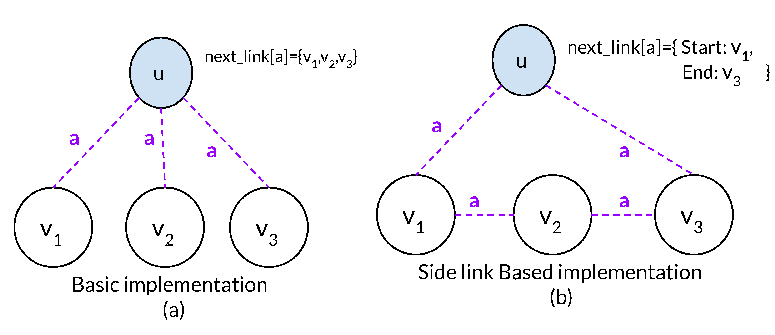
\includegraphics[width=\textwidth]{implementation}
\caption{Implementation of $next\_link$(s)} \label{figure:next_link_implementation}
\hfil
\end{figure*}

So, in summary, our proposed solutions are highly flexible and we can tweak different parts of it based on the requirements and constraints. 



\section*{Declarations}

Some journals require declarations to be submitted in a standardised format. Please check the Instructions for Authors of the journal to which you are submitting to see if you need to complete this section. If yes, your manuscript must contain the following sections under the heading `Declarations':

\begin{itemize}
\item Funding
\item Conflict of interest/Competing interests (check journal-specific guidelines for which heading to use)
\item Ethics approval 
\item Consent to participate
\item Consent for publication
\item Availability of data and materials
\item Code availability 
\item Authors' contributions
\end{itemize}

\noindent
If any of the sections are not relevant to your manuscript, please include the heading and write `Not applicable' for that section. 

%%===================================================%%
%% For presentation purpose, we have included        %%
%% \bigskip command. please ignore this.             %%
%%===================================================%%
\bigskip
\begin{flushleft}%
Editorial Policies for:

\bigskip\noindent
Springer journals and proceedings: \url{https://www.springer.com/gp/editorial-policies}

\bigskip\noindent
Nature Portfolio journals: \url{https://www.nature.com/nature-research/editorial-policies}

\bigskip\noindent
\textit{Scientific Reports}: \url{https://www.nature.com/srep/journal-policies/editorial-policies}

\bigskip\noindent
BMC journals: \url{https://www.biomedcentral.com/getpublished/editorial-policies}
\end{flushleft}



%%===========================================================================================%%
%% If you are submitting to one of the Nature Portfolio journals, using the eJP submission   %%
%% system, please include the references within the manuscript file itself. You may do this  %%
%% by copying the reference list from your .bbl file, paste it into the main manuscript .tex %%
%% file, and delete the associated \verb+\bibliography+ commands.                            %%
%%===========================================================================================%%



\begin{appendices}

\section{Section title of first appendix}\label{secA1}

An appendix contains supplementary information that is not an essential part of the text itself but which may be helpful in providing a more comprehensive understanding of the research problem or it is information that is too cumbersome to be included in the body of the paper.

%%=============================================%%
%% For submissions to Nature Portfolio Journals %%
%% please use the heading ``Extended Data''.   %%
%%=============================================%%

%%=============================================================%%
%% Sample for another appendix section			       %%
%%=============================================================%%

%% \section{Example of another appendix section}\label{secA2}%
%% Appendices may be used for helpful, supporting or essential material that would otherwise 
%% clutter, break up or be distracting to the text. Appendices can consist of sections, figures, 
%% tables and equations etc.

\end{appendices}


\bmhead{Acknowledgments}

Acknowledgments are not compulsory. Where included they should be brief. Grant or contribution numbers may be acknowledged.

Please refer to Journal-level guidance for any specific requirements.


\bmhead{Supplementary information}

If your article has accompanying supplementary file/s please state so here. 

Authors reporting data from electrophoretic gels and blots should supply the full unprocessed scans for key as part of their Supplementary information. This may be requested by the editorial team/s if it is missing.

Please refer to Journal-level guidance for any specific requirements.